\documentclass[12pt]{article}

\usepackage{listings}
\usepackage{hyphenat}
\usepackage{float}
\usepackage[T1]{fontenc}
\usepackage{hyperref,adjustbox}
\usepackage{graphicx}
\usepackage{pdfpages}
\usepackage[brazilian]{babel}
\usepackage{adjustbox}
\usepackage{multirow}
\usepackage{amssymb}
\usepackage{tabulary}
\usepackage{pifont}% http://ctan.org/pkg/pifont
\newcommand{\cmark}{\ding{51}}%
\newcommand{\xmark}{\ding{55}}%
\usepackage{tikz}
\usepackage{natbib}
\usepackage[T1]{fontenc}
\usepackage{bm}
\usepackage{enumitem}
\usepackage{algorithm}
%\usepackage{arevmath}     % For math symbols
\usepackage[noend]{algpseudocode}
\usepackage{mathtools}

\usepackage{titlesec}
\DeclarePairedDelimiter\ceil{\lceil}{\rceil}
\DeclarePairedDelimiter\floor{\lfloor}{\rfloor}

%\titleformat{\section}
%{\normalfont\Large\bfseries}{\thesection}{1em}{}[{\titlerule[0.8pt]}]

\usepackage{fontspec}
\setmainfont{QTPalatine}


\title{Trabalho Prático 3\\ Identificação de números primos usando computação paralela híbrida \\
	\large Computação Paralela}

\author{Heitor L. Werneck}
\begin{document}

\maketitle

\newpage
\tableofcontents

\newpage

\section{Introdução}
\subsection{Contextualização}

Um número primo é um número natural maior que 1 que não é produto de dois números naturais menores. Números naturais maiores que 1 que não são primos são chamados de número composto. A identificação de um número primo também tem relação com a função divisora do mesmo, já que os números primos tem exatamente 2 divisores exatos, então com o número de divisores exatos de um número é possível identificar a primalidade de um número (tarefa um pouco mais complexa que o teste de primalidade). Em matemática, e especificamente na teoria dos números, uma função divisora é uma função aritmética relacionada aos divisores de um inteiro. Quando referida como função divisora, ela conta o número de divisores de um inteiro (incluindo 1 e o próprio número). Diversas propriedades matemáticas podem ser observadas através da observação da função divisora ao longo de diferentes amostragens, que pode potencialmente auxiliar matemáticos nas suas áreas de pesquisas, e talvez até mesmo no caso de um algoritmo suficientemente eficiente pode ajudar a eliminar ou ''reforçar'' ainda mais corolários existentes na área.

Então o problema é simples, consiste em determinar o número de divisores exatos dos elementos $a_i$ de um vetor $A$ de tamanho $N$.


\subsection{Especificação do Problema}

O programa deverá ler o arquivo de entrada deverá e carregado para memoria no processo mestre. Após o processamento, cada processo escravo deverá retornar para o processo mestre quantos divisores exatos possui cada valor armazenado na sua fatia do vetor. Depois que o último escravo terminar, o processo mestre deverá colocar o número de divisores de cada elemento do arquivo de entrada em um arquivo de saída (saída.txt) na ordem em que os valores originais estavam no arquivo de entrada. A tomada de tempo das execuções será feita somente no processo mestre após leitura do arquivo de entrada e antes da escrita do arquivo de saída, ou seja, não será considerado o tempo de entrada/saída.

\subsection{Organização do Documento}

Nesse trabalho será feito a implementação paralela híbrida (memória compartilhada e distribuída) mestre-escravo usando MPI e OpenMP de um algoritmo que identifica números primos em um vetor de N inteiros. Nesse trabalho também é incluído, para o trabalho ser auto contido, a solução genérica, assim como no trabalho prático 1, na seção \ref{sec:solucao}. Após isso, na seção \ref{sec:solucao_paralela_hibrida}, é apresentado as justificativas, utilizando o perfil sequencial da solução serial, e a descrição da solução paralela híbrida. Na seção \ref{sec:implementacao} a documentação da implementação é apresentada, majoritariamente igual à apresentada no trabalho prático 1. Na seção \ref{sec:resultados_analises} os resultados da paralelização híbrida são apresentados, comparando com a versão paralela e serial do trabalho prático 1. Por fim, na seção \ref{sec:conclusao} é apresentado uma conclusão sobre o trabalho.


\section{Solução}
\label{sec:solucao}

Para solucionar esse problema procura-se inicialmente uma função/algoritmo $d(a_i)$ que consiga determinar o número de divisores de um elemento $a_i$.

Esse problema pode ser solucionado facilmente eficientemente com um algoritmo de fatoração de primos através da utilização da relação mostrada na Equação \ref{eq:divisorfunction}, que através da quantidade de vezes $e_i$ que um número primo aparece em uma fatoração de primos o número de divisores pode ser calculado. Isso é bem simples de entender, já que a fatoração de primos de um divisor $d'$ de $a$ tem que ser um subconjunto da fatoração de primos de $a$, então para o calculo do número de divisores basta calcular todos diferentes subconjuntos da fatoração de primos de um número $a$, o número de diferentes subconjuntos então são calculados usando a Equação \ref{eq:divisorfunction}.

\begin{equation}\label{eq:divisorfunction}
	d(a)=\prod_{i=1}^{k} (e_i+1)
\end{equation}

Agora para a fatoração de primos existem diversos métodos extremamente rebuscados, aqui será utilizado uma abordagem simples, porém de maneira otimizada. Para a fatoração e contagem de divisores será aplicado o algoritmo \ref{alg:divisorfunc} no qual uma lista de primos é percorrida (linha \ref{alg:divisorfunc:for}) e divisões são feitas caso o número seja um divisor e o contador de divisores e atualizado logo após as divisões (linha \ref{alg:divisorfunc:changes}). Para otimizar o método um limite de busca é estabelecido na linha \ref{alg:divisorfunc:end}, já que no caso de a condição ser atendida o número atual é um primo ou é o número 1, denotando que a fatoração pode ser finalizada. Note que nesta proposta não é guardado os fatores, já que não é isso que buscamos, mas sim o número de divisores do número.

\begin{algorithm}
	\caption{Função divisora\label{alg:divisorfunc}}
	\begin{algorithmic}[1]
		\Procedure{d}{$a,primes$}
		\State $num\_divisors\gets 1$
		\For{$i \gets 0$ to $|primes|-1$}\label{alg:divisorfunc:for}
		\State $count \gets 0$
		\If{$number \bm{\bmod} prime = 0$}\label{alg:divisorfunc:changes}
		\While{$number \bm{\bmod} prime = 0$}
		\State $number \gets number/prime$
		\State $count \gets count + 1$
		\EndWhile
		\State $num\_divisors \gets num\_divisors *(count+1)$
		\EndIf
		\If{$prime > \sqrt{number}$}\label{alg:divisorfunc:end}
		\If{$number \neq 1$}
		\State $num\_divisors \gets num\_divisors * 2$
		\EndIf
		\State \textbf{break}
		\EndIf
		\EndFor
		\State \Return $num\_divisors$
		\EndProcedure
	\end{algorithmic}
\end{algorithm}

Além disso ainda falta o gerador de primos que alimenta o algoritmo \ref{alg:divisorfunc} com uma lista de primos. Para gerar os primos até um limite $n$ foi implementado o crivo de eratóstenes com algumas otimizações para melhorar a performance do algoritmo. O crivo tradicional pode ser visto no algoritmo \ref{alg:erasto}. Na implementação duas otimizações, a primeira delas consiste de começar a marcação a partir do quadrado do primo encontrado e a segunda é a representação somente dos números impares do vetor, assim diminuindo o número de computações em dois e liberando mais memória (aumentando também a chance de cache hit).


\begin{algorithm}
	\caption{Crivo de Eratóstenes\label{alg:erasto}}
	\begin{algorithmic}[1]
		\Procedure{crivo}{$n$}
		\State $A[n+1]$ \Comment{Vetor de tamanho n}
		\State Atribua a todos elementos de $A$ o valor $true$
		\State $A[0]\gets 0; A[1]\gets 0$
		\For{$i \gets 2$ to $\sqrt{n}$}
		\If{$A[i] = true$}
		\State Atribua a todos múltiplos de $i$ até $n$ $false$
		\EndIf
		\EndFor
		\State primes \gets Transforme A em um vetor dos primos encontrados
		\State \Return primes
		\EndProcedure
	\end{algorithmic}
\end{algorithm}

O diagrama da figura \ref{fig:execoverviewserial} mostra uma visão geral de como cada componente desse se combina para resolver o problema final.

\begin{figure}[H]
	\centering
	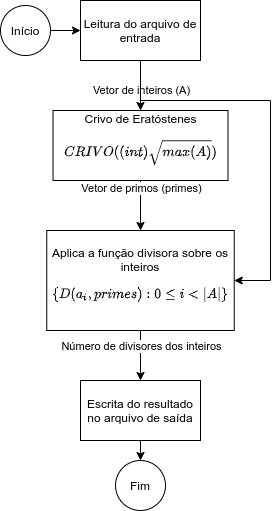
\includegraphics[width=4.5cm]{./overview_parallel_df.png}
	\caption{Visão geral da execução.}
	\label{fig:execoverviewserial}
\end{figure}

\section{Solução Paralela}
\label{sec:solucao_paralela_hibrida}

\subsection{Perfil de Desempenho Sequencial}

Com a execução da abordagem demonstrada anteriormente foi possível obter informações sobre oportunidades de paralelização. Abaixo o perfil de desempenho sequencial é apresentado. Na seção \ref{sec:implementacao} a cada uma dessas funções são apresentadas e descritas.


	{
		\scriptsize
		\begin{verbatim}
Each sample counts as 0.01 seconds.
  %   cumulative   self              self     total           
 time   seconds   seconds    calls   s/call   s/call  name    
 98.52     62.44    62.44 10000000     0.00     0.00  dfpack_df
  1.03     63.10     0.65        1     0.65     0.65  file_num_lines
  0.38     63.34     0.24        1     0.24    62.68  dfpack_serial_df
  0.21     63.47     0.13        1     0.13     0.13  write_result
  0.14     63.56     0.09        1     0.09     0.74  initial_setup
  0.08     63.61     0.05        1     0.05     0.05  get_max
  0.00     63.61     0.00        1     0.00     0.00  dfpack_prime_mask_to_vector
  0.00     63.61     0.00        1     0.00     0.00  dfpack_sieve_of_eratosthenes
\end{verbatim}
	}


Para essa avaliação do desempenho sequencial foi avaliado entradas com 1e7 amostras (números) obtidas de uma amostragem de 1e5 até 2e9 (com probabilidade uniforme), assim como no trabalho prático 1. Nesse perfil de desempenho do programa, é possível observar que a oportunidade de paralelização da chamada a função divisora pode representar um alto ganho de desempenho, visto que a maior parte do tempo é gasto nessa parte (98,52\% do tempo é gasto fazendo essa parte), assim como observado no trabalho prático 1. Essa função apresenta uma oportunidade de paralelização alta, por não apresentar dependência entre as chamadas. Outras porções do código não possuem essa característica, além de não apresentarem a mesma importância no tempo total de execução do programa.

\subsection{Proposta Paralela com MPI}

Aqui é apresentado a solução paralela proposta, apresentada primeiramente no trabalho prático 1. Se faz necessário apresentá-la de novo visto que a solução paralela híbrida somente faz pequenas modificações sobre esta.

A oportunidade mais em vista é a paralelização da aplicação da função divisora, que é uma parte da solução que é embaraçosamente paralela e pode ser aplicado uma abordagem mestre-escravo para melhorar o tempo de execução do algoritmo.

Em questão arquitetural, com o MPI, foi simplesmente feito uma abordagem mestre-escravo, no qual os escravos computam a função divisora em blocos determinados em tempo de execução, que são na prática blocos de tamanhos quase iguais para todos. Com esse método de decomposição de dados, os blocos foram divididos de acordo com as seguintes fórmulas, sendo id o identificador do processo, p o número de processos e n o tamanho total do bloco a ser decomposto.

Primeiro elemento controlado pelo processo id:

\begin{equation}
	\floor{\frac{id\cdot n}{p}}
\end{equation}

Último elemento controlado pelo processo id:

\begin{equation}
	\floor{\frac{(id+1)\cdot n}{p}}-1
\end{equation}

Para a paralelização no código foi especificamente modificado a linha 18 da função main do arquivo serial.c somente e algumas outras linhas necessárias para o setup do MPI dentro da própria main. A main foi modificada para comportar a configuração do nó mestre (envia e recebe dados) e os nós escravos (envia, recebe e computa). O mestre carrega o arquivo de entrada na memória e envia logo em seguida os blocos do mesmo no qual os escravos alocam dinamicamente o tamanho e processa-os para gerar os resultados finais.

A proposta de decomposição de dados nessa parte da computação pode trazer muitos ganhos por ser embaraçosamente paralela e também consegue escalar bem pelo mesmo motivo. Como mostrado no trabalho prático 1 com uma entrada grande o programa consegue escalar próximo do limite teórico de speed up pela natureza do problema, que não um baixo overhead de comunicação, é altamente paralelizável e etc.

Por fim, a figura \ref{fig:mpiparallel} mostra como a proposta funciona em um cluster de computadores.

\begin{figure}[H]
	\centering
	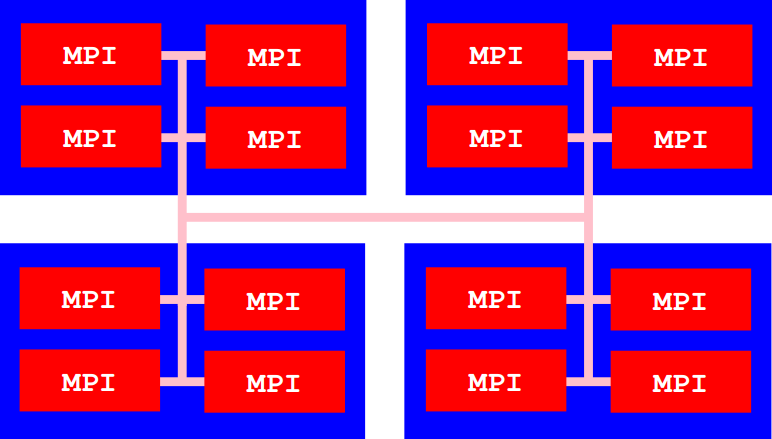
\includegraphics[width=0.7\linewidth]{./mpiparallel.png}
	\caption{Paralelização com MPI em um cluster de computadores.}
	\label{fig:mpiparallel}
\end{figure}


\subsection{Proposta Paralela Híbrida}

A proposta paralela híbrida consiste da utilização da proposta anterior para distribuição de blocos em diferentes nós de uma rede, para que uma computação distribuída seja possível. A visão geral da proposta pode ser vista na figura \ref{fig:hybridparallel}, que apresenta os escravos da proposta da paralelização híbrida.

\begin{figure}[H]
	\centering
	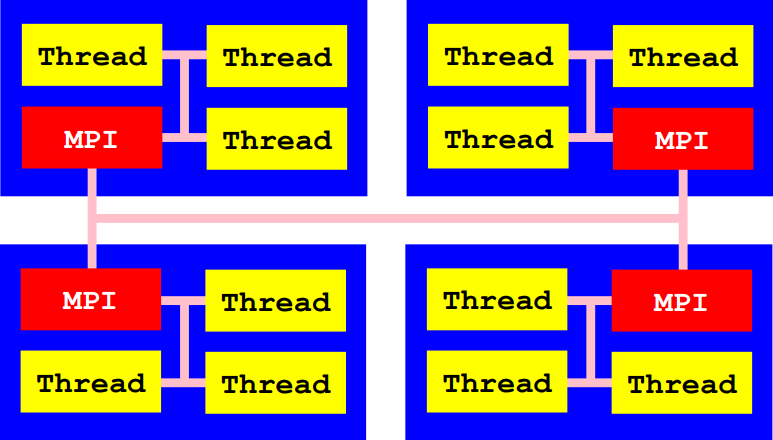
\includegraphics[width=0.7\linewidth]{./hybridparallel}
	\caption{Escravos da proposta de paralelização híbrida. Nesta figura só falta o mestre, que fica em um dos nós para distribuir as cargas de trabalho e não possui threads.}
	\label{fig:hybridparallel}
\end{figure}

Mais especificamente, nessa proposta cada escravo irá utilizar threads para realizar o cálculo do número de divisores exatos de um número em paralelo, já que essa foi a parte do código que apresentou maior potencial de paralelização. Ou seja, a função dfpack\_serial\_df será modificada para que no loop do cálculo do número de divisores exatos, isto seja feito de forma paralela utilizando o OpenMP.

A paralelização híbrida se adapta perfeitamente às arquiteturas atuais baseadas em clusters de multiprocessadores e/ou processadores multicore, pois induz menos comunicação entre os diferentes nós e em muitas situações aumenta o desempenho de cada nó sem ter que aumentar os requisitos de memória. Porém para a solução proposta, não espera-se ganhos significativos em relação a paralelização somente com MPI, pois o programa não é baseado em muitas comunicações, pois é embaraçosamente paralelo.

É esperado que essa solução seja minimamente superior a abordagem puramente com MPI somente em casos de problemas menores, no qual principalmente o overhead de criação dos processos e transferência de dados por meio de mais comunicações são mais relevantes. No caso de problemas maiores, devido a como o programa funciona, existe um overhead de entrada e saída no início para preparação da execução, logo o overhead da criação dos processos possivelmente terá menos impacto em problemas maiores. Além disso, nesses mesmos problemas menores se espera que a transferência de dados por meio de mais comunicações terá mais impacto no tempo total, até mesmo por conta do número de processos comunicantes, que pode fazer com que a solução híbrida seja superior a puramente MPI. Porém, por esse número de comunicações não crescer junto com o tamanho do problema, apenas a quantidade de dados a ser transferida, por ser embaraçosamente paralelo, espera-se que a solução híbrida não seja muito superior (possivelmente somente ganhos mínimos) a proposta somente com MPI em problemas maiores.


\section{Implementação}
\label{sec:implementacao}

Nessa seção será introduzido os módulos com suas respectivas funções, no caso desse problema não foi necessário a construção de nenhuma estrutura de dados. Os tipos primitivos foram suficientes para realizar toda implementação da solução.
\subsection{Módulo de Utilitários -- utils}

Esse é o módulo que contém as funções utilitárias dos programas, trata entrada e saída de dados assim como algumas transformações de dados.

\begin{enumerate}

	\item int file\_num\_lines(FILE *f)

	      Obtém o número de linhas de um arquivo e o retorna.

	\item int get\_max(int *vector, int num\_elements)

	      Obtém o máximo valor de um vetor de inteiros.

	\item int *initial\_setup(int argc, char **argv, int *num\_integers)

	      Gerência a configuração inicial dos programas, entrada e saída, parâmetros de entrada e leitura do arquivo de entrada.

	\item void write\_result(char *fout\_name, int *integers\_num\_divisors, int num\_integers)

	      Escreve o resultado final em um arquivo de saída.

\end{enumerate}

\subsection{ Módulo da Função Divisora -- dfpack}

Este pacote provê os algoritmos que envolvem a solução para o problema, como o crivo de Eratóstenes, a função divisora e etc.

\begin{enumerate}
	\item int *dfpack\_prime\_mask\_to\_vector(bool *primes\_mask, int primes\_mask\_size, int num\_primes)

	      Transforma um vetor de booleano que identifica números primos para um vetor de inteiros que contém todos os primos não marcados (true) no vetor de booleano. É usado para transformar o resultado do crivo de Eratóstenes.

	\item int *dfpack\_sieve\_of\_eratosthenes(int limit, int *num\_primes)

	      Implementação do crivo de eratóstenes otimizada com a remoção de números pares e com marcação rápida descrita anteriormente. limit é o número para limitar a pesquisa de primos. num\_primes retorna o número de primos encontrados no limite fornecido. Essa função retorna um vetor de inteiros com os números primos encontrados.

	\item int dfpack\_df(int number, int *primes, int num\_primes)

	      Função divisora que dá o número de divisores exatos de um número. Recebe um número, uma lista de primos e a quantidade de primos na lista (tamanho da mesma). A função retorna o número de devisores exatos de um número como dito anteriormente.

	\item int *dfpack\_serial\_df(int *integers, int max\_number, int num\_integers)

	      Função que gerência todo processo para calcula a função do divisor para vários números inteiros. Para isso ela trata de executar o crivo de Eratóstenes antes e depois executa a função divisora para inteiro da lista de inteiros passada e depois retorna uma lista com o número de divisores de cada elemento. Para a solução paralela híbrida essa função possui uma diretiva para paralelização do loop que chama a função divisora.

\end{enumerate}

\subsection{Implementação serial -- serial.c}

Esse é um dos códigos principais, chamado serial.c, que contém a implementação principal do programa serial. O mesmo utiliza as duas bibliotecas descritas anteriormente para solucionar o problema de maneira serial.


\subsection{Implementação paralela -- parallel.c}

Esse é um dos códigos principais, chamado parallel.c, que contém a implementação principal do programa paralelo. O mesmo utiliza as duas bibliotecas descritas anteriormente para solucionar o problema de maneira paralelo e faz algumas modificações relativas ao código serial que segue um fluxo mais simples de execução. Além disso, como foi implementado a solução paralela híbrida, esse mesmo programa é utilizado para essa implementação, no qual quando compilado com a \textit{flag} PARALLEL, a solução híbrida é gerada.

\section{Resultados e Análises}
\label{sec:resultados_analises}

Nesta seção é inicialmente apresentado um resultado de uma execução simples do programa, após isso é apresentado um teste de vazamento de memória, que foram feitos no trabalho prático 1. Por fim, é apresentado resultados da paralelização híbrida, comparando com resultados dos algoritmos do trabalho prático 1.

\subsection{Execução}

Primeiramente, a seguir é mostrado um simples caso de entrada e saída do programa que demonstra como o mesmo funciona e como se comporta. Veja a seguir a execução do programa sequencial:

\begin{verbatim}
$ ./serial-df ./data/entrada.txt ./data/saida.txt  
Time spend with computation: 0.005838

$ pr -m -t ./data/entrada.txt ./data/saida.txt | head
entrada.txt                         saida.txt
109988769                           16
12440600                            48
208049563                           8
81673565                            4
98418805                            4
56478723                            20
145841961                           8
48805077                            8
39824052                            12
113904704                           14
\end{verbatim}

É possível ver que nenhum desses números são primos, pois nenhum deles possui 2 como saída (2 divisores, que no caso seria o próprio número e o número 1). As saídas foram todas extensivamente testadas com uma biblioteca do Python (arith-lib) e nenhuma incongruência foi observada.

\subsection{Memória}

Para verificação de qualquer vazamento de memória foi utilizado o \textit{Valgrind}. Como pode ser visto abaixo, em uma execução normal não existe qualquer problema em relação a vazamento de memória com o programa.

	{
		\scriptsize
		\begin{verbatim}
==279131== Memcheck, a memory error detector
==279131== Copyright (C) 2002-2017, and GNU GPL'd, by Julian Seward et al.
==279131== Using Valgrind-3.17.0 and LibVEX; rerun with -h for copyright info
==279131== Command: ./serial-df ./data/entrada.txt ./data/saida.txt
==279131== 
Time spend with computation: 0.097611
==279131== 
==279131== HEAP SUMMARY:
==279131==     in use at exit: 0 bytes in 0 blocks
==279131==   total heap usage: 10 allocs, 10 frees, 37,573 bytes allocated
==279131== 
==279131== All heap blocks were freed -- no leaks are possible
==279131== 
==279131== For lists of detected and suppressed errors, rerun with: -s
==279131== ERROR SUMMARY: 0 errors from 0 contexts (suppressed: 0 from 0)
\end{verbatim}
	}

Além disso, o programa paralelo não foi possível ser testado, dado que o próprio MPI ou mais especificamente Open-MPI possui vazamentos de memória até mesmo em execuções simples, o que dificulta a utilização do \textit{Valgrind}. Apesar disso o código foi extensivamente revisado e não possui nenhum vazamento de memória aparente.

\subsection{Resultados da Paralelização}

Para avaliar os ganhos da paralelização híbrida feita é importante a utilizar em um ambiente real de cluster de computadores. Para esse trabalho foi utilizado três computadores em uma rede local. Como estes computadores não tinham um sistema de arquivos distribuídos foi encontrado alguns inconvenientes na execução neste ambiente. Para resolver isso foi utilizado uma abordagem com Docker Swarm que utiliza o sistema operacional Alpine Linux, apresentada em um artigo do IEEE CCWC \cite{nguyen2017distributed}\footnote{\url{https://github.com/NLKNguyen/alpine-mpich}}. A abordagem proposta neste paper foi adaptada, com uma versão mais recente do sistema operacional e alguns outros ajustes para o caso de uso deste trabalho. A imagem do Docker utilizada para realização dos experimentos está disponível no Docker Hub \footnote{\url{https://hub.docker.com/repository/docker/heitor57/df-mpi}}, além da versão modificada da proposta do paper \footnote{\url{https://hub.docker.com/repository/docker/heitor57/alpine-mpich}}.

Os conjuntos de dados utilizados são variações do apresentado na subseção de desempenho sequencial, com diferentes quantidades de números na entrada (i.e., 1e4, 1e5, 1e6 e 1e7).

A tabela \ref{tab:results} apresenta os tempos de computação dos algoritmos. A abordagem serial apresentou resultados significativamente piores que as outras, como esperado, mesmo no menor conjunto de dados (i.e., t1e4). Apesar disso, no conjunto de dados t1e4 foi onde a abordagem serial teve seu melhor resultado comparado com os outros métodos. Por conta de ser uma base de dados menor a eficiência do algoritmo paralelo diminui muito bruscamente, como pode ser visto na tabela \ref{tab:results_eficiencia}. A eficiência é uma medida do uso da capacidade computacional. Ela mede a proporção entre o desempenho e o número de recursos disponíveis para atingir esse desempenho.

Além disso, os algoritmos paralelos, apresentados nas colunas P (paralelo somente com MPI) e HP (paralelo híbrido), apresentaram speed ups próximos do linear quando a carga de trabalho foi alta. Apesar disso, os resultados foram afetados por conta da execução em cluster, que não foi feita no trabalho prático 1, e o speed up ficou minimamente menor quando o número de escravos total é igual ao do trabalho prático 1, um resultado esperado. Fora isto, esperava-se um resultado de speed up um pouco mais próximo do linear devido a solução paralela não apresentar dependências, mas em trabalhos futuros pode ser abordado a execução com uma maior carga de trabalho ou números em grandezas maiores (necessitaria uma adaptação do código para esse caso, para representar números maiores) para avaliar o impacto.

No geral foi possível observar que a proposta paralela híbrida conseguiu ganhar da paralela que usa somente MPI por diferenças mínimas nas tabelas \ref{tab:results}, \ref{tab:results_speedup} e \ref{tab:results_eficiencia} que não são significativas. Apesar disso, entende-se que isso se deu por conta dos overheads que são minimizados com a solução que combina paralelismo em memória compartilhada e distribuída. Caso a solução proposta tivesse mais dependências na paralelização, então seria esperado que a solução híbrida obtivesse mais ganhos. Como não é esse o caso, assim como previsto na seção \ref{sec:solucao_paralela_hibrida}, o algoritmo não apresenta ganhos significativos sobre a versão puramente MPI, visto também aqueles cenários no qual o overhead da criação de processos não faz muita diferença como discutido na seção \ref{sec:solucao_paralela_hibrida}.


Como pode ser visto na tabela \ref{tab:results_speedup} o speed up máximo foi de 9 e 10 considerando somente 12 processos ou threads (P4 e HP4) que trabalham na computação dos resultados efetivamente (desconsiderando o nó mestre).


\begin{table}[H]
	\footnotesize
\begin{adjustbox}{center}
	\begin{tabular}{|c|c|ccc|ccc|}
		\hline
		Entrada & S         & P2       & P3       & P4       & HP2       & HP3      & HP4      \\
		\hline
		t1e4    & 0.069453  & 0.013431 & 0.011433 & 0.019427 & 0.015432  & 0.013598 & 0.010617 \\
		t1e5    & 0.651358  & 0.116043 & 0.083666 & 0.064406 & 0.11115   & 0.089641 & 0.071479 \\
		t1e6    & 5.415279  & 1.140077 & 0.789125 & 0.620157 & 1.123055  & 0.786196 & 0.613554 \\
		t1e7    & 53.750999 & 10.94354 & 7.436622 & 5.652318 & 10.941552 & 7.389212 & 5.603844 \\
		\hline
	\end{tabular}
      \end{adjustbox}
	\caption{Tempo de execução em segundos do algoritmo sequencial (S), paralelo (P) e paralelo híbrido (HP) com diferentes quantidades processos escravos (2, 3 e 4) ou threads (2, 3 e 4) em cada máquina do cluster.}
	\label{tab:results}
\end{table}

\begin{table}[H]
	\footnotesize
\begin{adjustbox}{center}
	\begin{tabular}{|c|ccc|ccc|}
		\hline
		Entrada & P2       & P3       & P4       & HP2       & HP3      & HP4      \\
		\hline
		t1e4    & 5.1711  & 6.07478 &  3.57508 & 4.50058 & 5.10759 & 6.54168 \\
		t1e5    & 5.61307 & 7.78522 & 10.1133  & 5.86017 & 7.2663  & 9.11258 \\
		t1e6    & 4.74992 & 6.86238 &  8.73211 & 4.82192 & 6.88795 & 8.82608 \\
		t1e7    & 4.91166 & 7.22788 &  9.50955 & 4.91256 & 7.27425 & 9.59181 \\
		\hline
	\end{tabular}
      \end{adjustbox}
	\caption{Speed up do algoritmo paralelo (P) e paralelo híbrido (HP) com diferentes quantidades processos escravos (2, 3 e 4) ou threads (2, 3 e 4) em cada máquina do cluster.}
	\label{tab:results_speedup}
\end{table}

\begin{table}[H]
	\footnotesize
\begin{adjustbox}{center}
	\begin{tabular}{|c|ccc|ccc|}
		\hline
		Entrada & P2       & P3       & P4       & HP2       & HP3      & HP4      \\
		\hline
		t1e4    & 0.861849 & 0.674976 & 0.297923 & 0.750097 & 0.56751  & 0.54514  \\
		t1e5    & 0.935512 & 0.865024 & 0.842776 & 0.976695 & 0.807366 & 0.759382 \\
		t1e6    & 0.791654 & 0.762487 & 0.727676 & 0.803653 & 0.765328 & 0.735507 \\
		t1e7    & 0.818611 & 0.803098 & 0.792462 & 0.81876  & 0.80825  & 0.799317 \\
		\hline
	\end{tabular}
      \end{adjustbox}
	\caption{Eficiência do algoritmo paralelo (P) e paralelo híbrido (HP) com diferentes quantidades processos escravos (2, 3 e 4) ou threads (2, 3 e 4) em cada máquina do cluster.}
	\label{tab:results_eficiencia}
\end{table}


%Agora finalmente será abordado os ganhos obtidos com a paralelização e análises de alguns resultados obtidos. Pela tabela é possível ver que de acordo com o aumento do número de processos na versão paralela "P2", "P3", "P4", e etc há também a diminuição do tempo, em todas as bases parece ter um speed up máximo de 10x com 24 processos. Apesar de ainda não ser próximo do speed up teórico é uma boa melhora. Também é importante notar que como a arquitetura é mestre-escravo quando há 2 processos é quase a mesma coisa que o serial.

%\begin{table}[H]
	%\tiny
	%\begin{tabular}{|c|ccccccc|}
		%\hline
		%Entrada & S         & P2        & P3        & P4        & P8       & P16      & P24      \\
		%\hline
		%1e4     & 0.06722   & 0.065067  & 0.030805  & 0.021386  & 0.01734  & 0.00832  & 0.006639 \\
		%1e5     & 0.641231  & 0.640219  & 0.286639  & 0.188591  & 0.139259 & 0.076519 & 0.050823 \\
		%1e6     & 5.366242  & 5.270993  & 2.722727  & 1.832781  & 0.807689 & 0.749196 & 0.493886 \\
		%1e7     & 52.446117 & 52.784925 & 26.903649 & 18.206626 & 8.040143 & 7.457124 & 4.9046   \\
		%\hline
	%\end{tabular}
	%\caption{Algoritmo sequêncial e paralelo com diferentes quantidades de processos em paralelo.}
%\end{table}


\section{Conclusão}
\label{sec:conclusao}

Com este trabalho foi possível ter uma melhor ideia sobre como utilizar o MPI e OpenMP na prática e seus possíveis ganhos. A abordagem de paralelização híbrida (memória compartilhada e distribuída) foi explorada e exercitada na prática. As duas abordagens de paralelização, com MPI (especificamente Open-MPI) e OpenMP se mostraram práticas para utilização em ambientes reais.

Os três algoritmos implementados (i.e., serial, paralelo e híbrido paralelo) foram avaliados pelo tempo de execução, speed up e eficiência. Os resultados obtidos não demonstraram ganhos significativos da abordagem puramente MPI comparado com a abordagem híbrida (utilizando MPI e OpenMP). Isso se deu pela natureza da solução paralela proposta (i.e., embaraçosamente paralela), que não apresenta dependência e não necessita de comunicação entre os \textit{workers}, deste modo os ganhos da solução híbrida são limitados. Apesar disso as abordagens paralelas tiveram ganhos significativos sobre a serial, chegando a 9.5 de speed up.

\bibliographystyle{plainnat}
\bibliography{doc.bib}
\end{document}
